We refer to the \textit{ansatz} as the quantum-circuit structure, \textit{i.e.} the layout defining quantum-gates placements. While such a word stand for \textit{an educated guess or an additional assumption made to help solve a problem}~\cite{wikiansa}, let us remark that trainability and noise-related issues make it non-trivial to define what an \textit{educated guess} for a given problem is in the NISQ-era.

We will make a distinction between \textit{fixed}-structured ansatzes (\textit{i.e.} where $\kvec$ is fixed), and \textit{variable}-structure ones, in which also the structure of the circuit is optimized. In the latter case, the optimization is arguably more complex, since it consists on finding the right circuit structure on top of the continuous parameter optimization.

A key parameter that characterizes the ansatz is the number of gates present in the circuit. It is thus essential to construct ansatzes that maintain this number as low as possible to mitigate noise and trainability-related issues, but also that have enough expressibility to contain the problem solution (or at least an approximate version of it).

In the following we will first discuss some commonly-used fixed-structured ansatzes, and we will then turn to the variable-structure case.
% \subsubsection{Fixed-structure ansatzes}\label{sssec:blabla}

\vspace{1cm}

Let us now discuss on some commonly-used fixed-structure ansatzes. We first consider a \textit{separable} ansatz as depicted in Fig.~\ref{fig:FANSATZ}. Here, the structure is so trivial that no entanglement is generated by the circuit, since only local operations are performed on each qubit. Assuming that the initial state is separable ---we often consider it to be $\ket{0}^{\otimes n}$---, only a very small fraction of the Hilbert space can be reached under this circuit's choice~\cite{separableAnna}, and the overall performance is expected to be poor since the presence of entanglement is generally required. Also, note that the separable case can efficiently be simulated in a classical computer, and thus we do would not expect them to provide any quantum advantage.

\begin{figure}[t!]
    \centering
    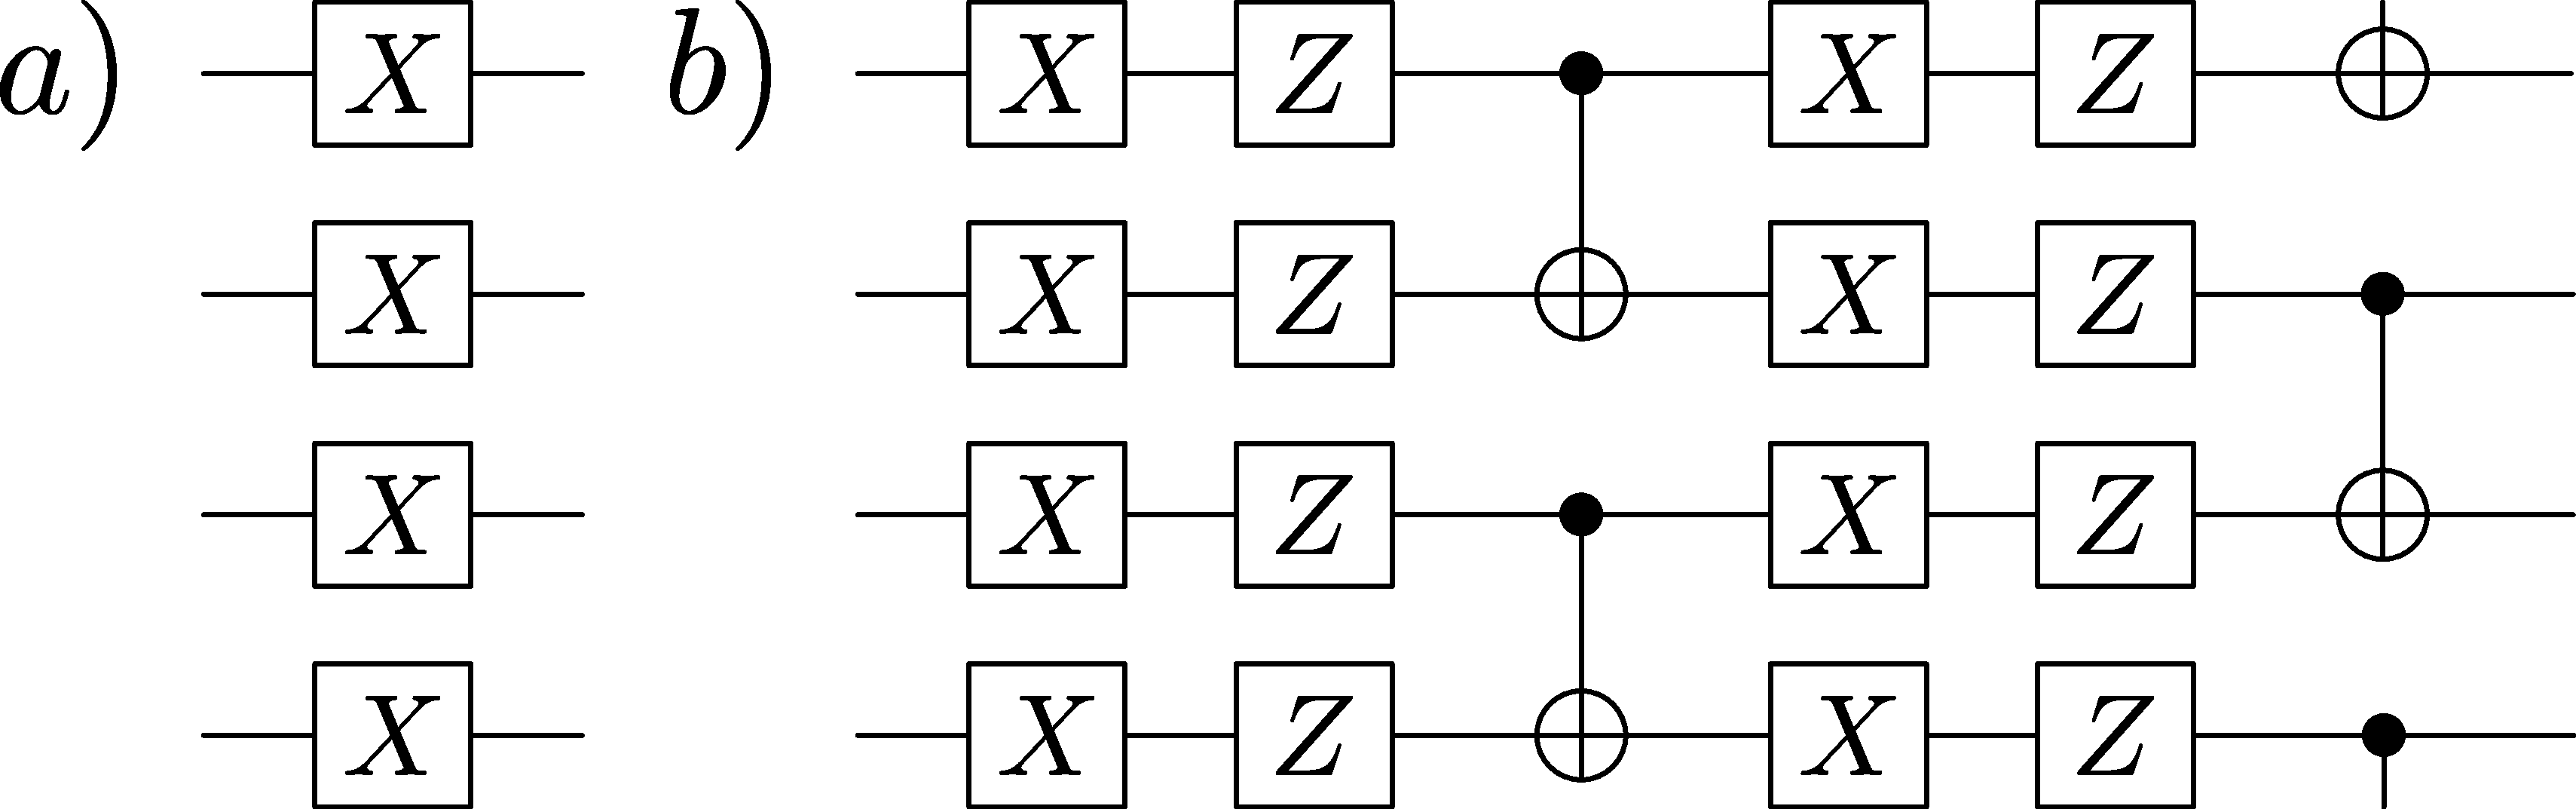
\includegraphics[width=1.\textwidth]{Figures/VANS/Fig2.pdf}
    \caption{We show examples of commonly-used quantum circuits. In \textit{(a)} we depict a separable product ansatz which generates no entanglement between the qubits. On the other hand, \textit{(b)} shows two layers of a shallow alternating Hardware Efficient Ansatz where neighboring  qubits are initially entangled.  Here $Z$ ($X$) indicates a parametrized rotation about the $z$ ($x$) axis (the angles $\bm{\theta}$ are not explicitely shown, but such are the degree of freedom to optimize over).}
    \label{fig:FANSATZ}
\end{figure}

This issue can be addressed with the layered Hardware Efficient Ansatz\cite{kandala2017hardware}, which we refer as HEA. Here, the gates are arranged in a brick-like fashion and act on alternating pairs of qubits, as depicted in Fig.~\ref{fig:FANSATZ}. We define a $L$-HEA as a circuit in which $L$ layers are stacked next to each other: a single layer consists on $n-1$ two-qubit gates (in the figure, rotations around $x$ and $z$ axis, followed by a CNOT) that correlate two neighbour qubits in the circuit. We here will consider the qubits as a cyclic chain, where the bottom one is also conected to the upper one, although this definition can be adapted to specific qubit-connection constraints of the quantum computer at hand. As $L$ increases, it can be expected that HEA becomes more expressible. as opposed to the separable circuit, whose expressibility is very poor.

In turn, HEA turns out to be \textit{too} expressible~\cite{holmes2021connecting}, in the sense that any unitary can be mimicked using enough HEA-layers, and this can lead to trainability issues. For a sufficiently-expressible PQC, the landscape of possible unitaries $\mathcal{U}$ that can be reached by varying its parameters turns to be hard to navigate, in the sense that the cost-function landscape becomes very flat, a phenomenon known as a \textit{barren plateau}. The latter fact constitute a big challenge for an optimization proccedure that needs to navigate such landscape and reach the lowest cost-function value, as discussed in Sec.~\ref{ssec:1_nisq_barrenplateaus}.

One of the main advantages of HEA is that it employs gates native to the specific device used, hence avoiding an unnecessary overhead in the number of gates present in the circuit, arising from compiling non-native unitaries into native gates (for instance, the building-blocks in the figure could be replaced with gates coming from another dictionary). This type of ansatz is \textit{problem-agnostic}, in the sense that it is expressible enough so that it can be generically employed for any task; in Chapter~\ref{chapter:VANS} we will often use this ansatz for benchmarking purposes.

On the other hand, a hint on the solution for the target problem to be solved by a quantum computer can, in principle, be helpful when building the ansatz. This claim should certainly holds in the ideal (\textit{e.g.} noise-less) scenario, and in VQAs, this is reflected by the so-called \textit{problem-inspired} ansatzes. Here the goal is to encode information of the problem into the ansatz's structure so the optimal solution of Eq.~\eqref{eq:optimization} exists within the parameter space without requiring high expressibility.

An example of such fixed-structure ansatzes is the Quantum Alternating Operator Ansatz (QAOA) for optimization problems, which is aimed to adiabatically prepare the ground-state of a \textit{problem}-hamiltonian, and thus alternates between a \textit{mixing} unitary and a \textit{problem} one. We will not discuss thse ansatzes here, and the interested reader can find more details in Refs.~\cite{farhi2014quantum,hadfield2019quantum}.

On a different note, considerable effort has been made in order to construct physically-inspired ansatzes in the field of quantum chemistry, and the Unitary Coupled Cluster (UCC) Ansatz~\cite{cao2019quantum,bartlett2007coupled} is an example of them. We will discuss the quantum-chemistry problem in greater detail in Sec.~\ref{ssec:molecular_ham_vans}. Essentially, we here seek to prepare the ground state of a molecular Hamiltonian, which (under the Born-Oppenheimer approximation) translates to solve a many-body fermionic system, known as the \textit{electronic-structure problem}.
While much insight from the classical methods that tackle this problem can be brought to the NISQ scenario, some issues raise up. Namely, we need to map the [UCC] ansatz from fermions to qubits, as well as the molecular Hamiltonian, since we are here targeting applications on digital quantum computers. Such mapping can be done by the Jordan-Wigner transform (or alternatively Bravi-Kitaev). Unfortunately, this ussually comes with an overhead in the number of quantum gates required to build the specific circuit (and also a large number of Pauli observables to represent the molecular Hamiltonian). This fact constitutes a big challenge for NISQ applications, since deep circuits are severely affected by noise.

We might think of quantum chemistry as a subset of problems that quantum computing can potentially addess. Generally, for a given physical problem, a family of quantum-circuit structures reflecting certain symmetries of potential solutions could in principle be constructed. However, quantum-hardware noise makes it highly no trivial to directly translate such physical intuition into the structure of the quantum circuit. %, since the afforementioned challenges related to noise generally arise.
\vspace{1cm}

Under the presence of limited resources, each component of the VQA that could in principle be optimized over, should be optimized over. This constitutes the spirit behind several efforts~\cite{grimsley2019adaptive,tang2019qubit,zhang2021mutual, rattew2019domain,chivilikhin2020mog, cincio2021machine, cincio2018learning,du2020quantum,zhang2020differentiable} to adapt the circuit layout to the specific scenario at hand (\textit{e.g.} a noise model, or the restricted availability of quantum hardware). In the following we will review some of such efforts, which are known as \textit{variable-structure ansatzes}. We remark that this is not the end of the story regarding optimization of VQA's components. As a matter of fact, we could also optimize the way cost-function estimates are obtained~\cite{algorithmiq1,algorithmiq2}, though we will only focus to optimizing circuit's structure.

The overall strategy of variable-structure ansatzes consists of iteratively changing the quantum circuit by placing (or removing) gates that empirically lower the cost-function value after the continuous-parameter optimization. The first proposal for variable ansatzes for quantum chemistry was introduced in~\cite{grimsley2019adaptive} under the name of ADAPT-VQE. Here, the authors follow a circuit structure similar to that used in the UCC ansatz introduced above, and propose to iteratively grow the circuit by appending gates that implement fermionic operators chosen from a pool of single and double excitation operators. At each iteration, one decides which operator in the pool is to be appended, which can lead to a considerable overhead if the number of operators in the pool is large. Similarly to the UCC case, the mapping from fermions to qubits can lead to prohibitively deep circuits. This issue can be overcomed using the qubit-ADAPT-VQE~\cite{tang2019qubit} algorithm, where the pool of operators is modified in such a way that only easily implementable gates are considered. However, the size of the pool still grows with the number of qubits. We refer the reader to~\cite{claudino2020benchmarking} for a detailed comparison between ADAPT-VQE and UCC ansatzes.

A different approach to variable-structure ansatzes that has gained considerable attention are machine-learning-aided evolutionary algorithms (EA) that upgrade individuals (quantum circuits) from a population. Noticeably, the presence of quantum correlations makes it so that it is not straightforward to combine features between circuits during the evolution, as simply merging two promising circuits does not necessarily lead to low cost-function values. Thus, only random mutations have been considered so far. An example of this method is found in the
Evolutionary VQE (EVQE)~\cite{rattew2019domain}, where one explores the Hilbert space \textit{smoothly} by growing the circuit with identity-initialized blocks of gates and randomly removing sequences of gates. Another example of an evolutionary algorithm is the Multi-objective Genetic VQE (MoG-VQE)~\cite{chivilikhin2020mog}, where one uses building blocks that are randomly placed along the circuit, and simultaneously optimizes both the energy and number of entangling gates. Evolutionary algorithms constitute a promising approach to ansatzes design, they nevertheless come at the cost of high quantum-computational resources to evolve populations of quantum circuits.

In addition, in Refs.~\cite{du2020quantum,zhang2020differentiable,pirhooshyaran2021quantum,du2020quantum} tools from auto-machine were employed in order to learn how to build ansatzes. The overall idea behind these methods is that of employing neural network (supernet) that suggests the quantum circuit structure; supernet-training can be done using policy-gradient methods, a variant of the reinforcement-learning algorithms that we consider in Sec.~\ref{sec:1_rl}. While the idea of artificial-intelligence improving (quantum) neural-network architectures is exciting, it is extremely resource-consuming: recall that the amount of data required to train a neural network is very often prohibitively high. Similarly to the EA case, the high amount of resources consumed by this method is a challenge that needs to be addressed.

Finally, in Refs.~\cite{cincio2018learning,cincio2021machine} a methodology, formalized by the VAns algorithm~\cite{bilkis2021semi} --- \textit{i.e.} our main contribution to the field, and explained and showcased in great detail in Chapter~\ref{chapter:VANS} --- was used to obtain a short-depth version of a given unitary under specific quantum hardware constraints (such as connectivity, noise-model as represented by quantum channels or available gates). %Explaining and showcasing our algorithm will be the matter of Chapter~\ref{chapter:VANS}.

Having reviewed some commonly-used quantum circuit structures, we will now turn to discuss the continuous optimization.
